% PDF-only book front matter for the modern edition.
% The exterior cover is followed by the usual interior opening pages:
% half-title, frontispiece, full title, edition notice, then contents.

% Flag the paged modern edition so the shared source can omit the duplicate
% flowing-output photograph later in frontmatter-modern.tex.
\NewDocumentCommand{\WaveModernBookFrontMatter}{}{}
\NewCommandCopy{\WaveModernOriginalTableOfContents}{\tableofcontents}

% Exterior cover. It is intentionally outside the Roman-numbered preliminaries.
\WaveModernCover
\clearpage
\nopagecolor

% Count the opening pages in the usual way while suppressing folios on
% the half-title, frontispiece, title, and edition-notice pages. Contents begins
% visibly on page v.
\pagenumbering{roman}

% Half-title (i)
\thispagestyle{empty}
\begin{center}
	\vspace*{2.45in}
	{\sffamily\color{WaveAccent}\fontsize{25}{30}\selectfont\bfseries
		WAVE MOTIONS IN THE OCEAN\par}
\end{center}
\clearpage

% Frontispiece (ii)
\thispagestyle{empty}
\begin{center}
	\vspace*{0.62in}
	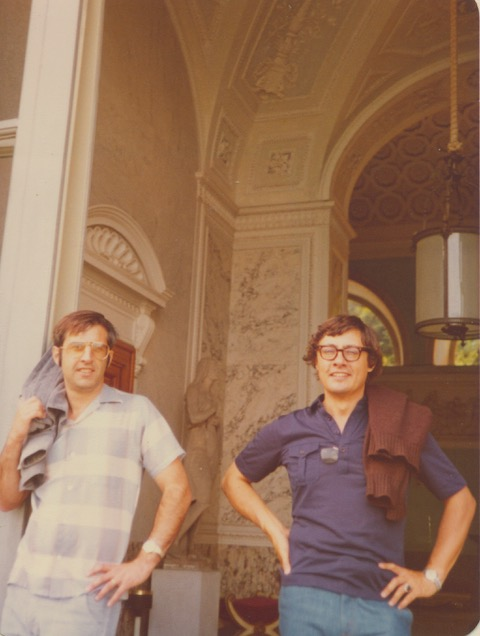
\includegraphics[width=0.68\linewidth]{images/salmon-hendershott-como-1980.jpg}
	\par\smallskip
	{\small Rick Salmon (left) and Myrl Hendershott at Villa Carlotta, Lake Como,
		during the International School of Physics ``Enrico Fermi,'' Course LXXX,
		\textit{Topics in Ocean Physics}, July 1980.\par}
\end{center}
\clearpage

% Full title page (iii)
\thispagestyle{empty}
\begin{center}
	\vspace*{0.82in}
	{\sffamily\color{WaveAccent}\fontsize{28}{32}\selectfont\bfseries
		WAVE MOTIONS IN THE OCEAN\par}
	\vspace{0.20in}
	{\fontsize{18}{22}\selectfont\itshape Myrl's View\par}
	\vspace{0.78in}
	{\large \textit{Presented to} \textbf{Myrl C. Hendershott}\par}
	\vfill
	{\large \textbf{David C. Chapman and Paola Malanotte-Rizzoli}\par}
	\vspace{0.10in}
	{\normalsize August 1989\par}
	\vfill
	{\normalsize Edited by \textbf{Albert M. W. Yau}\par}
	\vspace{0.10in}
	{\normalsize August 2026\par}
\end{center}
\clearpage

% Copyright / edition-notice verso (iv). Do not claim ownership of the
% original lecture notes; record authorship, edition details, license, and cover
% credit instead.
\thispagestyle{empty}
\vspace*{2.25in}
{\footnotesize
	\noindent\textit{Wave Motions in the Ocean: Myrl's View}\par
	\noindent David C. Chapman and Paola Malanotte-Rizzoli. Presented to
	Myrl C. Hendershott, August 1989.\par
	\medskip
	\noindent Edited by Albert M. W. Yau, August 2026.\par
	\smallskip
	\noindent Digital edition build:
	\href{\wavebuildurl}{\texttt{\wavebuildlabel}}.\par
	\medskip
	\noindent This digital edition has been authorized by Paola Malanotte-Rizzoli
	for release under the Creative Commons Attribution-NonCommercial-ShareAlike
	4.0 International license (CC BY-NC-SA 4.0).\par
	\medskip
	\noindent The original source scan was preserved on James Pringle's website.\par
}
\wavecovercredit
\clearpage

% Contents begins on the first page with a visible Roman folio (v).
\WaveModernOriginalTableOfContents
\clearpage

% frontmatter-modern.tex keeps a source-level \tableofcontents for the
% generated README/HTML pipeline. Suppress that later duplicate in the PDF.
\RenewDocumentCommand{\tableofcontents}{}{}
